\section{Functionalities Implemented to satisfy requirements}
For each of the required entities we have implemented PHP functions to Create, Read, Update and Delete a resource. These functions are placed in our Ressource controllers which handle the requests coming from the front end to our API. To make our live's simpler we have implemented the following helper functions accessible by all the rest of our controllers.
\begin{minted}{php}
<?php
public function doInsertAndGetId($tableName, Collection $parameters){
        $keys = $parameters->keys()->join(',');
        $placeholders = $parameters->map(function () { return '?';})->join(',');
        $result = DB::insert("INSERT INTO $tableName (
                $keys
            ) VALUES ($placeholders)",
            [
                ...$parameters->values(),
            ]
        );
        if ($result) {
            $id = DB::getPdo()->lastInsertId();
            return $id;
        }
        return null;
    }
    
\end{minted}

\begin{minted}{php}
<?php
public function doUpdate($tableName, $key, $id, Collection $fieldsToUpdate){
        $values = $fieldsToUpdate->values();
        $values->push($id);
        return DB::update("UPDATE $tableName SET {$fieldsToUpdate->keys()->join(',')} WHERE $key = ?", $values->toArray());
    }
\end{minted}

\begin{minted}{php}
<?php
public function syncGroupIds($personId, $groupZones)
    {
        $toDelete = collect();
        $toAdd = collect();

        if (!$personId) {
            abort(500);
        }

        // delete anything that isn't in the group_zones
        $dbGroupIds = collect(DB::select("SELECT gzp.group_id FROM GroupZonePersonPivot gzp
	            WHERE person_id = '{$personId}'"))->pluck('group_id')->toArray();
        foreach ($dbGroupIds as $dbGroupId) {
            if (!in_array($dbGroupId, $groupZones)) {
                $toDelete->push($dbGroupId);
            }
        }
        foreach ($groupZones as $groupZone) {
            if (!in_array($groupZone, $dbGroupIds)) {
                $toAdd->push($groupZone);
            }
        }
        if ($toAdd->isNotEmpty()) {
            $stringAdd = $toAdd->map(function ($groupId) use (&$personId) {
                return "($personId,$groupId)";
            })->join(',');
            DB::insert("INSERT INTO GroupZonePersonPivot (`person_id`, `group_id`)
                VALUES $stringAdd");
        }
        if ($toDelete->isNotEmpty()) {
            $toDelete->map(function ($id) use (&$personId) {
                DB::insert("DELETE FROM GroupZonePersonPivot WHERE person_id=$personId and group_id=$id");
            });
        }
    }
\end{minted}
\subsection{Patient CRUD}
\subsubsection{Create}
\begin{minted}{php}
<?php
public function create(Request $request){
        $parameters = collect($request->only([
            'medicare',
            'first_name',
            'last_name',
            'address',
            'postal_code',
            'postal_code_id',
            'citizenship',
            'email',
            'phone',
            'dob'
        ]));
        $parameters['medicare'] = str_replace(' ', '' , $parameters['medicare']);
        $parameters->put('password', bcrypt(str_replace('-','',$parameters['dob'])));
        $parameters->put('api_token', Str::random(60));
        $id = $this->doInsertAndGetId('Person', $parameters);
        $this->syncGroupIds($id, $request->group_zones);
        DB::insert("INSERT INTO Patient (person_id) VALUES (?)", [$id]);
        return response()->json(['patient_id' => $id], $id ? Response::HTTP_CREATED : Response::HTTP_BAD_REQUEST);
}
    
\end{minted}
\subsubsection{Read}
\begin{minted}{php}
<?php
 public function readAll(Request $request){
        return response()->json(DB::select("SELECT p.patient_id, ps.*
            FROM Patient p
            JOIN Person ps ON p.person_id = ps.person_id"));
}

 public function readOne($id){
        $result = DB::select("SELECT
                p.patient_id,
                ps.*,
                c.city,
                pv.province,
                r.region_name,
                GROUP_CONCAT(gzp.group_id) as 'group_zones'
            FROM Patient p
            JOIN Person ps ON p.person_id = ps.person_id
            LEFT JOIN GroupZonePersonPivot gzp ON gzp.person_id = p.person_id
            JOIN PostalCode pc ON ps.postal_code_id = pc.postal_code_id
            JOIN City c ON pc.city_id = c.city_id
            JOIN Region r ON c.region_id = r.region_id
            JOIN Province pv ON pv.province_code = r.province_code
            WHERE p.patient_id = '{$id}'
            GROUP BY p.patient_id");

        return response()->json((count($result) > 0 ? $result[0] : null),
            count($result) > 0 ? 200 : 404
        );
}

\end{minted}

\subsubsection{Update}
\begin{minted}{php}
<?php
 public function update(Request $request, $id){
        $personFieldsToUpdate = collect();

        if ($request->filled('password')) {
            $personFieldsToUpdate->put('password = ?', $request->password);
        }
        if ($request->filled('first_name')) {
            $personFieldsToUpdate->put('first_name = ?', $request->first_name);
        }
        if ($request->filled('last_name')) {
            $personFieldsToUpdate->put('last_name = ?', $request->last_name);
        }
        if ($request->filled('address')) {
            $personFieldsToUpdate->put('address = ?', $request->address);
        }
        if ($request->filled('postal_code_id')) {
            $personFieldsToUpdate->put('postal_code_id = ?', $request->postal_code_id);
        }
        if ($request->filled('citizenship')) {
            $personFieldsToUpdate->put('email = ?', $request->email);
        }
        if ($request->filled('email')) {
            $personFieldsToUpdate->put('phone = ?', $request->phone);
        }
        if ($request->filled('phone')) {
            $personFieldsToUpdate->put('phone = ?', $request->phone);
        }
        if ($request->filled('dob')) {
            $personFieldsToUpdate->put('dob = ?', $request->dob);
        }
        $personId = DB::select("SELECT person_id FROM Patient WHERE patient_id = '{$id}'")[0]->person_id ?? null;
        if (!$personId) {
            abort(500);
        }
        $this->syncGroupIds($personId, $request->group_zones);
        $this->doUpdate('Person', 'person_id', $id, $personFieldsToUpdate);
        $fieldsUpdated = $personFieldsToUpdate->count();
        return response()->json(['message' => $fieldsUpdated . " field(s) updated successfully!"], 200);
}

\end{minted}
\subsubsection{Delete}
\begin{minted}{php}
<?php
public function delete($id){
        $status = DB::delete("DELETE FROM Patient WHERE patient_id = ?", [$id]);
        return response()->json(['status' => "Deleted successfully!"], 200);
}

\end{minted}

\subsection{Public Health Worker CRUD}
\subsubsection{Create}
\begin{minted}{php}
<?php
public function create(Request $request){
        $parameters = collect($request->only([
            'medicare',
            'password',
            'first_name',
            'last_name',
            'address',
            'postal_code_id',
            'citizenship',
            'email',
            'phone',
            'dob',
            'region_id'
        ]));
        $pid = $this->doInsertAndGetId('Person', $parameters);

        $this->syncGroupIds($pid, $request->group_zones);
        $schedule = $request->input('schedule');
        $position_id = $request->input('position_id');
        $center_id = $request->input('health_center_id');

        DB::insert("INSERT INTO PublicHealthWorker (person_id, position_id, schedule, health_center_id) VALUES (?,?,?,?)", [$pid, $position_id, $schedule, $center_id]);
    }
\end{minted}
\subsubsection{Read}
\begin{minted}{php}
<?php
 public function readAll(Request $request){
        $stringSearch = "SELECT w.health_worker_id, pst.position, w.schedule, ps.*
            FROM PublicHealthWorker w
            JOIN Position pst ON w.position_id = pst.position_id
            JOIN Person ps ON w.person_id = ps.person_id
            JOIN PublicHealthCenter phc ON w.health_center_id = phc.health_center_id";

        if ($request->filled("health_center_id")) {
            $stringSearch .= " WHERE w.health_center_id = " . $request->health_center_id;
        }
        return response()->json(DB::select($stringSearch));
}
    public function readOne($id){
        $result = DB::select("SELECT
                w.health_worker_id,
                pst.position,
                w.schedule,
                ps.*,
                c.city,
                p.province,
                r.region_name,
                GROUP_CONCAT(gzp.group_id) as 'group_zones'
            FROM PublicHealthWorker w
            JOIN Position pst ON w.position_id = pst.position_id
            JOIN Person ps ON w.person_id = ps.person_id
            LEFT JOIN GroupZonePersonPivot gzp ON gzp.person_id = ps.person_id
            JOIN PostalCode pc ON ps.postal_code_id = pc.postal_code_id
            JOIN City c ON pc.city_id = c.city_id
            JOIN Region r ON c.region_id = r.region_id
            JOIN Province p ON p.province_code = r.province_code
            WHERE w.health_worker_id = '{$id}'
            GROUP BY w.health_worker_id");

        return response()->json((count($result) > 0 ? $result[0] : null),
            count($result) > 0 ? 200 : 404
        );
}

\end{minted}

\subsubsection{Update}
\begin{minted}{php}
<?php
 public function update(Request $request, $id){
        $personFieldsToUpdate = collect();
        $workerFieldsToUpdate = collect();
        if ($request->filled('password')) {
            $personFieldsToUpdate->put('password = ?', $request->password);
        }
        if ($request->filled('first_name')) {
            $personFieldsToUpdate->put('name = ?', $request->name);
        }
        if ($request->filled('last_name')) {
            $personFieldsToUpdate->put('last_name = ?', $request->name);
        }
        if ($request->filled('address')) {
            $personFieldsToUpdate->put('address = ?', $request->address);
        }
        if ($request->filled('postal_code_id')) {
            $personFieldsToUpdate->put('postal_code_id = ?', $request->postal_code_id);
        }
        if ($request->filled('citizenship')) {
            $personFieldsToUpdate->put('email = ?', $request->email);
        }
        if ($request->filled('email')) {
            $personFieldsToUpdate->put('phone = ?', $request->phone);
        }
        if ($request->filled('phone')) {
            $personFieldsToUpdate->put('phone = ?', $request->phone);
        }
        if ($request->filled('dob')) {
            $personFieldsToUpdate->put('dob = ?', $request->dob);
        }
        if ($request->filled('region_id')) {
            $personFieldsToUpdate->put('region_id = ?', $request->region_id);
        }
        if ($request->filled('position')) {
            $workerFieldsToUpdate->put('position = ?', $request->position);
        }
        if ($request->filled('schedule')) {
            $workerFieldsToUpdate->put('schedule = ?', $request->dob);
        }
        $personId = DB::select("SELECT person_id FROM PublicHealthWorker WHERE health_worker_id = '{$id}'")[0]->person_id ?? null;
        $this->syncGroupIds($personId, $request->group_zones);
        $this->doUpdate('Person', 'person_id', $id, $personFieldsToUpdate);
        $this->doUpdate('PublicHealthWorker', 'health_worker_id', $id, $workerFieldsToUpdate);
        $fieldsUpdated = $personFieldsToUpdate->count() + $workerFieldsToUpdate->count();
        return response()->json(['message' => $fieldsUpdated . " field(s) updated successfully!"], 200);
}

\end{minted}

\subsubsection{Delete}
\begin{minted}{php}
<?php
public function delete($id){
        $status = DB::delete("DELETE FROM PublicHealthWorker WHERE health_worker_id = ?", [$id]);
        return response()->json(['status' => "Deleted successfully!"], 200);
}

\end{minted}
\subsection{Facility CRUD}
\subsubsection{Create}
\begin{minted}{php}
<?php
public function create(CreateFacilityRequest $request){
        $parameters = collect($request->only([
            'name',
            'phone',
            'address',
            'postal_code',
            'postal_code_id',
            'type',
            'website',
            'method',
            'drive_thru'
        ]));
        $id = $this->doInsertAndGetId('PublicHealthCenter', $parameters);
        return response()->json(['health_center_id' => $id], $id ? Response::HTTP_CREATED : Response::HTTP_BAD_REQUEST);
}
\end{minted}
\subsubsection{Read}
\begin{minted}{php}
<?php
public function readAll(Request $request){
        return response()->json(DB::select("SELECT `health_center_id`, `name`, `phone`, `address`, `type`,`method`,`drive_thru` FROM PublicHealthCenter"));
}
public function readAll(Request $request){
     return response()->json(DB::select("SELECT `health_center_id`, `name`, `phone`, `address`, `type`,`method`,`drive_thru` FROM PublicHealthCenter"));
}
\end{minted}
\subsubsection{Update}
\begin{minted}{php}
<?php
public function create(CreateFacilityRequest $request){
        $parameters = collect($request->only([
            'name',
            'phone',
            'address',
            'postal_code',
            'postal_code_id',
            'type',
            'website',
            'method',
            'drive_thru'
        ]));
        $id = $this->doInsertAndGetId('PublicHealthCenter', $parameters);
        return response()->json(['health_center_id' => $id], $id ? Response::HTTP_CREATED : Response::HTTP_BAD_REQUEST);
}
\end{minted}
\subsubsection{Delete}
\begin{minted}{php}
<?php
public function create(CreateFacilityRequest $request){
        $parameters = collect($request->only([
            'name',
            'phone',
            'address',
            'postal_code',
            'postal_code_id',
            'type',
            'website',
            'method',
            'drive_thru'
        ]));
        $id = $this->doInsertAndGetId('PublicHealthCenter', $parameters);
        return response()->json(['health_center_id' => $id], $id ? Response::HTTP_CREATED : Response::HTTP_BAD_REQUEST);
}
\end{minted}
\subsection{Region CRUD}
\subsubsection{Create}
Our Webapp already has all the regions we don't create or delete any and we have an autocomplete function that renders the region based on postal code.
\begin{minted}{php}
<?php
public function autocomplete(Request $request){
        return response()->json(DB::select("
            SELECT pc.postal_code_id, c.city_id, c.city, r.region_id, r.region_name, p.province_code, p.province
            FROM PostalCode pc
            JOIN City c ON pc.city_id = c.city_id
            JOIN Region r ON c.region_id = r.region_id
            JOIN Province p ON p.province_code = r.province_code
            WHERE pc.`postal_code_id` like '{$request->input('postal_code')}%'"));
}
\end{minted}
\subsubsection{Read}
\begin{minted}{php}
<?php
public function readAll(Request $request){
        return response()->json(DB::select("
            SELECT
                r.region_id,
                r.region_name,
                a.alert_id,
                a.alert_info,
                GROUP_CONCAT(c.city) as 'cities',
                GROUP_CONCAT(pc.postal_code_id) as 'postal_codes'
            FROM Region r
            JOIN Alert a ON r.alert_id = a.alert_id
            JOIN City c ON c.region_id = r.region_id
            JOIN PostalCode pc ON pc.city_id = c.city_id
            GROUP BY r.region_id"));
}
 public function readOne($id)
    {
        $result = DB::select("SELECT * FROM Region WHERE $id = region_id");

        return response()->json((count($result) > 0 ? $result[0] : null),
            count($result) > 0 ? 200 : 404);
    }
    
\end{minted}

\subsubsection{Update}
\begin{minted}{php}
<?php
public function update(Request $request, $id){
        $newAlertId = $request->input('alert_id');
        $currentAlertId = DB::select("SELECT alert_id FROM Region WHERE region_id = $id")[0]->alert_id ?? null;
        try {
            if (abs($newAlertId - $currentAlertId) > 1 && $newAlertId != 0 || !$currentAlertId) {
                return response()->json(['message' => " wowow cant jump from more than 1 alert my guy!"], 400);
            } else {
                $this->doUpdate('Region', 'region_id', $id, collect(['alert_id = ?' => $newAlertId]));
                $fieldsUpdated = 1;
                return response()->json(['message' => $fieldsUpdated . " field(s) updated successfully!"], 200);
            }
        } catch (QueryException $e) {
            if ($e->getCode() == 23000) {
                return  response()->json(['message' => "alert does not exist!"], 400);
            }
        }
    }
\end{minted}

\subsection{Group-Zone CRUD}
\subsubsection{Create}
\begin{minted}{php}
<?php
 public function create(Request $request){
        $parameters = collect($request->only([
            'name',
            'activity',
        ]));
        $id = $this->doInsertAndGetId('GroupZone', $parameters);

        return response()->json(['group_zone_id' => $id], $id ? Response::HTTP_CREATED : Response::HTTP_BAD_REQUEST);
}
\end{minted}
\subsubsection{Read}
\begin{minted}{php}
<?php
public function readAll(Request $request){
        return response()->json(DB::select("SELECT * FROM GroupZone"));
}
    public function readOne($id){
        $result = DB::select("SELECT *
            FROM GroupZone WHERE group_id = '{$id}'");
        return response()->json((count($result) > 0 ? $result[0] : null),
            count($result) > 0 ? 200 : 404);
}

\end{minted}
\subsubsection{Update}
\begin{minted}{php}
<?php
public function update(Request $request, $id){
        $groupZoneFieldsToUpdate = collect();
        
        if ($request->filled('activity')) {
            $groupZoneFieldsToUpdate->put('activity = ?', $request->activity);
        }
        if ($request->filled('name')) {
            $groupZoneFieldsToUpdate->put('name = ?', $request->name);
        }
        $this->doUpdate('GroupZone', 'group_id', $id, $groupZoneFieldsToUpdate);
        $fieldsUpdated = $groupZoneFieldsToUpdate->count();
        return response()->json(['message' => $fieldsUpdated . " field(s) updated successfully!"], 200);
}
\end{minted}
\subsection{Recommendation CRUD}
\subsubsection{Create}
\begin{minted}{php}
<?php
 public function create(Request $request){
 $recommendation = $request->input('recommendation');
 DB::insert("INSERT INTO Recommendation (recommendation) VALUES (?)", [$recommendation]);
}
\end{minted}
\subsubsection{Read}
\begin{minted}{php}
<?php
public function readAll(Request $request){
        return response()->json(DB::select("
            SELECT
                r.region_id,
                r.region_name,
                a.alert_id,
                a.alert_info,
                GROUP_CONCAT(c.city) as 'cities',
                GROUP_CONCAT(pc.postal_code_id) as 'postal_codes'
            FROM Region r
            JOIN Alert a ON r.alert_id = a.alert_id
            JOIN City c ON c.region_id = r.region_id
            JOIN PostalCode pc ON pc.city_id = c.city_id
            GROUP BY r.region_id"));
}
public function readOne($id){
        $result = DB::select("SELECT * FROM Region WHERE $id = region_id");

        return response()->json((count($result) > 0 ? $result[0] : null),
            count($result) > 0 ? 200 : 404);
}

\end{minted}
\subsubsection{Update}
\begin{minted}{php}
<?php
public function update(Request $request, $id){
        $field  = $request->input('recommendation');
        DB::update("UPDATE recommendation  SET recommendation = (?) WHERE recommendation_id = $id", [$field]);

}
\end{minted}
\begin{minted}{php}
<?php
public function update(Request $request, $id){
        $newAlertId = $request->input('alert_id');
        $currentAlertId = DB::select("SELECT alert_id FROM Region WHERE region_id = $id")[0]->alert_id ?? null;
        try {
            if (abs($newAlertId - $currentAlertId) > 1 && $newAlertId != 0 || !$currentAlertId) {
                return response()->json(['message' => " wowow cant jump from more than 1 alert my guy!"], 400);
            } else {
                $this->doUpdate('Region', 'region_id', $id, collect(['alert_id = ?' => $newAlertId]));
                $fieldsUpdated = 1;
                return response()->json(['message' => $fieldsUpdated . " field(s) updated successfully!"], 200);
            }
        } catch (QueryException $e) {
            if ($e->getCode() == 23000) {
                return  response()->json(['message' => "alert does not exist!"], 400);
            }
        }
    }
    
\end{minted}

\subsection{Trigger for Alerts}
Once a new alert is set for a region, a trigger must send message(s) to all the people that
are registered in that region informing them of the new alert state, and also inform them
whether the alert is more strict or less strict than the previous alert
\subsubsection{MySQL}
\begin{minted}{MYSQL}
CREATE TRIGGER alertTrigger
AFTER UPDATE ON Region
FOR EACH ROW
BEGIN
if (NEW.alert_id = 4) THEN
INSERT INTO messages(`message`, `region_id`, `msg_date`,`person_id`, `alert_id`)
SELECT 
  CONCAT('Bonsoir ',ps.first_name, ', email: ', ps.email, ' this is an automated message generated at ',NOW(),' to warn you that the alert level in your region: ', r.region_name,' went from ', a.alert_info, ' to ', b.alert_info, 
  '.This is RED alert, the maximum alert a region can have. Please follow the link and read about guidelines, visit www.coviddb.com/guidelines.') AS 'message',
  OLD.region_id AS 'region_id',
  NOW() AS 'msg_date',
  ps.person_id AS 'person_id',
  NEW.alert_id AS 'alert_id'
FROM 
  Person ps
  JOIN PostalCode pc ON pc.postal_code_id = ps.postal_code_id
  JOIN City c ON c.city_id = pc.city_id
  JOIN Region r ON r.region_id = OLD.region_id
  JOIN Alert a ON a.alert_id = OLD.alert_id
  JOIN Alert b ON b.alert_id = NEW.alert_id;
  END IF;
  if (NEW.alert_id < 4) THEN
INSERT INTO messages(`message`, `region_id`, `msg_date`,`person_id`, `alert_id`)
SELECT 
  CONCAT('Bonsoir ',ps.first_name, ', email: ', ps.email, ' this is an automated message generated at ',NOW(),' to warn you that the alert level in your region: ', r.region_name,' went from ', a.alert_info, ' to ', b.alert_info) AS 'message',
  OLD.region_id AS 'region_id',
  NOW() AS 'msg_date',
  ps.person_id AS 'person_id',
  NEW.alert_id AS 'alert_id'
FROM 
  Person ps
  JOIN PostalCode pc ON pc.postal_code_id = ps.postal_code_id
  JOIN City c ON c.city_id = pc.city_id
  JOIN Region r ON r.region_id = OLD.region_id
  JOIN Alert a ON a.alert_id = OLD.alert_id
  JOIN Alert b ON b.alert_id = NEW.alert_id;
  END IF;
END; 
\end{minted}

\subsection{Trigger for Diagnostic Result}
Upon a person’s test result is determined, a trigger must send a message to the person notifying him/her of the test result. If the test is positive, an additional message is sent to the person with information about the public health recommendations, and a reminder message is sent to the person to fill out the follow-up-form using the username (medicare card number) and the password (DOB of the form ddmmyyyy).
\subsubsection{MySQL}
\begin{minted}{MYSQL}
CREATE TRIGGER diagTrigger
AFTER INSERT ON Diagnostic
FOR EACH ROW
BEGIN
IF (NEW.result = 1) THEN
INSERT INTO messages(`message`, `region_id`, `msg_date`,`person_id`, `alert_id`)
SELECT 
  CONCAT('Bonsoir ', ps.first_name, '. You have received a POSITIVE result for your COVID diagnostic.'),
  null AS 'region_id',
  NEW.diagnostic_date AS 'msg_date',
  ps.person_id AS 'person_id',
  null AS 'alert_id'
FROM 
  Person ps
  JOIN patient pc ON pc.person_id = ps.person_id AND NEW.patient_id = pc.patient_id;
    INSERT INTO messages(`message`, `region_id`, `msg_date`,`person_id`, `alert_id`)
SELECT 
  CONCAT('Bonsoir ', ps.first_name, '. You have recently received a POSITIVE diagnostic for COVID-19. Here are the public health recommendations that should be followed during 
  14 consecutive day after your diagnostic www.coviddb.com/recommendations. Reminder: Do not forget to fill up the follow-up-form on www.coviddb.com using your medicare <', ps.medicare, '> as username and your date of birth <', ps.dob, '> as password.'),
  null AS 'region_id',
  NEW.diagnostic_date AS 'msg_date',
  ps.person_id AS 'person_id',
  null AS 'alert_id'
FROM 
  Person ps
  JOIN patient pc ON pc.person_id = ps.person_id AND NEW.patient_id = pc.patient_id;
  END IF;
IF (NEW.result = 0) THEN
INSERT INTO messages(`message`, `region_id`, `msg_date`,`person_id`, `alert_id`)
SELECT 
  CONCAT('Bonsoir ', ps.first_name, '. You have received a NEGATIVE result for your COVID diagnostic.'),
  null AS 'region_id',
  NEW.diagnostic_date AS 'msg_date',
  ps.person_id AS 'person_id',
  null AS 'alert_id'
FROM 
  Person ps
  JOIN patient pc ON pc.person_id = ps.person_id AND NEW.patient_id = pc.patient_id;
  END IF;
END;
\end{minted}



\section{Scripts \& Queries}

%  Q8  % 
\subsection{Form Followup}
Fill-Up a follow up form for a person who is tested positive, for fourteen consecutive days following the test results. The form must include the date, the time, the temperature, the status of all the main symptoms and other symptoms as specified for the COVID-19 as well as other non-specified symptom(s) if exists. Every person can fill up his/her form using the username and password. The username is the medicare card number of the person and the password is the date of birth of the person of the form (ddmmyyyy).
\subsubsection{MySQL}
\begin{minted}{MYSQL}
INSERT INTO FollowUpForm(`filled_by`, `patient_id`, `form_id`, `created_at`, `temperature`,`other_symptoms`)
VALUES (5,2,1,'2021-04-11 02:26:25', `36`,`strong_appetite`);
INSERT INTO FollowUpFormSymptomPivot (`form_id`, `symptom_id`) 
SELECT '1', symptom_id
FROM Symptoms 
WHERE symptom IN ('fever','loss_of_appetite');
\end{minted}

\subsubsection{PHP}
The implementation in the back-end is written as:\\
\begin{minted}{php}
<?php
# Q9
public function create(Request $request){
        $parameters = collect($request->only([
            'filled_by',
            'patient_id',
            'form_id',
            'created_at',
        ]));
        DB::insert("INSERT INTO FollowUpForm (filled_by, patient_id, form_id, created_at) VALUES (?,?,?,?)", [$parameters]);
}
\end{minted}
\subsubsection{Representative tuples}
\begin{table}[ht]
\centering
\begin{tabular}{|l|l|l|l|} 
        \hline
        filled\_by & patient\_id & form\_id & created\_at \\
        \hline 
        1&1& 17 & 2021-04-16 10:25:27 \\
        1&1 & 25 & 2021-04-17 10:30:00\\
        1&1 & 39 & 2021-04-18 21:07:18\\
        5&1 & 42 & 2021-04-19 10:25:27\\
        1&1 & 58 & 2021-04-20 04:00:00\\
        \hline
\end{tabular}
\caption{Follow-up form representative tuples}
\end{table}
\subsubsection{Screenshot in WebApp}    
\begin{figure}[h]
    \centering
    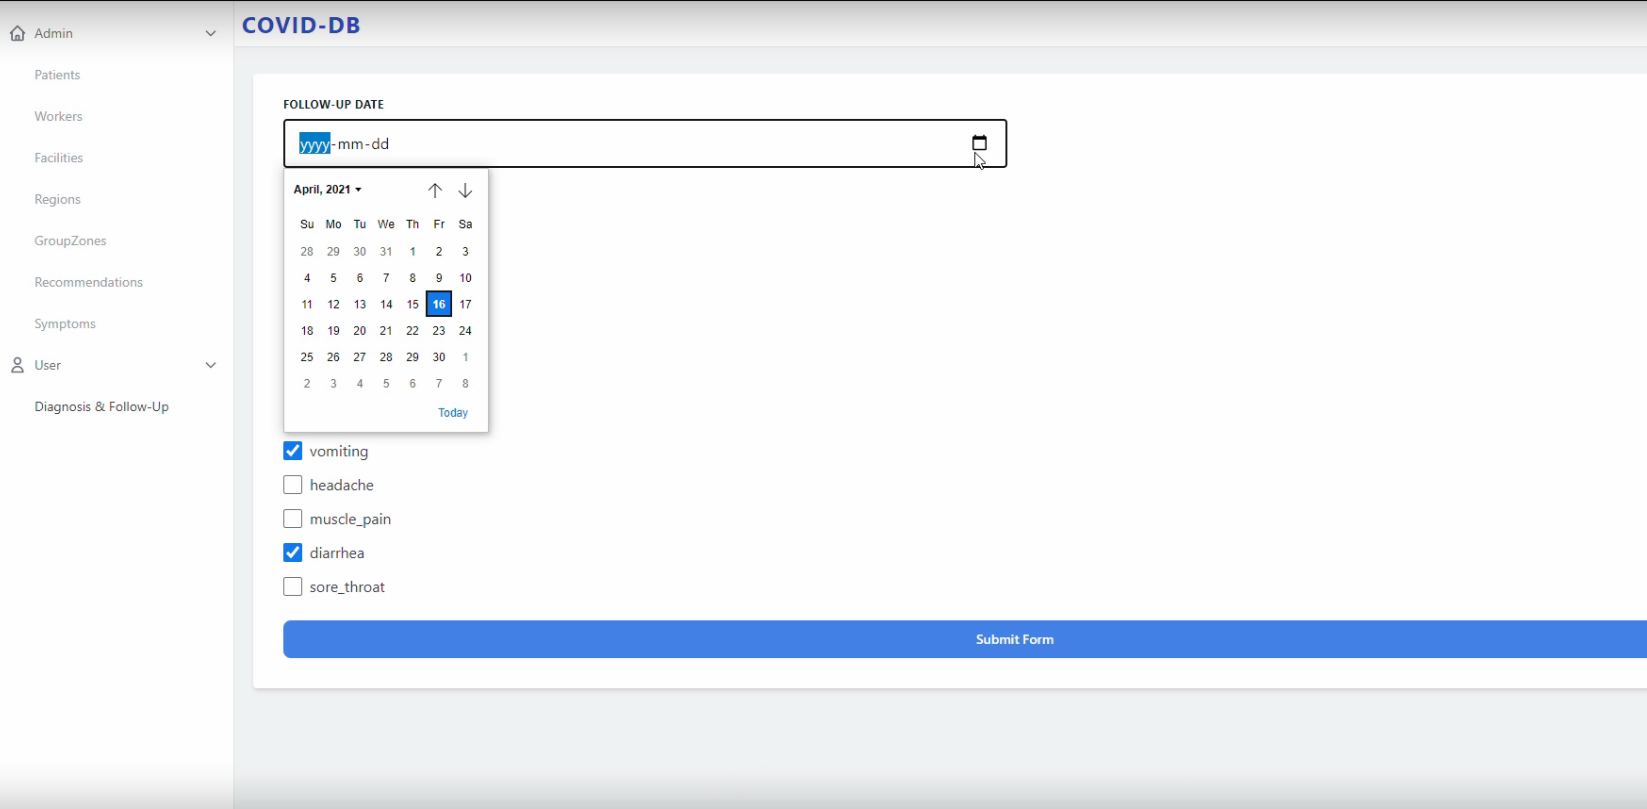
\includegraphics[scale=0.35]{imgs/fillingAForm.PNG}
    \caption{Filling up a form}
\end{figure}


\newpage

%  Q9  % 
\subsection{Symptoms Progress}
Provide a detail progress of all the symptoms for a given person who tested positive on a specific date.
\subsubsection{MySQL}

\begin{minted}{MYSQL}
SELECT (`form_id`),(`patient_id`),(`created_at`),(`symptom`)
FROM followupformsymptompivot 
NATURAL JOIN followupform
NATURAL JOIN symptom 
WHERE patient_id = patient_id AND created_at > start_date
\end{minted}

\subsubsection{PHP}
The implementation in the back-end is written as:
\begin{minted}{php}
<?php
# Q9
public function readAll(Request $request){
return response()->json(DB::select("SELECT (`form_id`),(`patient_id`),(`created_at`),(`symptom`)
FROM followupformsymptompivot 
NATURAL JOIN followupform
NATURAL JOIN symptom 
WHERE patient_id = $request->patient_id AND created_at = $request->start_date"));
}
\end{minted}

\subsubsection{Representative tuples}
An example GET request would be : \\
127.0.0.1:8000/api/form?patient\_id=1\&start\_date='2021-04-17'\\
Which would return something like :
\begin{table}[ht]
\centering
\begin{tabular}{|l|l|l|l|} 
        \hline
        form\_id & patient\_id & created\_at & symptom \\
        \hline 
        4&1& 2021-04-17 10:25:27 & headache\\
        5&1 & 2021-04-18 10:25:27 & throat ache\\
        6&1 & 2021-04-18 21:07:18 & cough\\
        7&1 & 2021-04-18 10:30:00 & cough\\
        8&1 & 2021-04-19 11:00:00 & headache\\
        \hline
\end{tabular}
\caption{Symptom progress representative tuples}
\end{table}
%  Q10  % 
\subsection{Messages during a given time} 
Display all messages generated by the system within a specific period of time.

\subsubsection{MySQL}
\begin{minted}{MYSQL}
SELECT * FROM Messages 
WHERE msg_date > start_date 
AND msg_date < end_date
\end{minted}

\subsubsection{PHP}
The implementation in the back-end is written as:
\begin{minted}{php}
<?php
# Q10
public function readAll(Request $request){
        return response()->json(DB::select("SELECT * FROM messages WHERE msg_date > $request->start_date AND msg_date < $request->end_date"));
}

\end{minted}

\subsubsection{Representative tuples}
An example GET request would be : \\
127.0.0.1:8000/api/messages?start\_date='2021-04-13 23:59:59'\&end\_date=2021-04-17 23:59:59'\\
Which would return something like :
\begin{table}[ht]
    \centering
    \begin{tabular}{|l|l|l|l|l|l|l|} 
        \hline
        msg\_id  & region\_id & msg\_date & alert\_id\ & message & person\_id \\
        \hline 
        45 & NULL & 2021-04-14 15:56:50 & NULL & \multicolumn{1}{m{6cm}|}{Bonsoir Eliott You have recieved a POSITIVE result for you COVID diagnostic.
        Please click here to view the public health recommendations that should be followed \& click here to fill your followup form for the 14 next days} & 6  \\
        46 & NULL & 2021-04-15 15:56:50 & NULL & \multicolumn{1}{m{6cm}|}{Bonsoir Angela. You have recieved a Negative result for you COVID diagnostic.} & 1 \\
       47 & 21 & 2021-04-15 19:06:50 & 4 & \multicolumn{1}{m{6cm}|}{Bonsoir Tyrell. This is an automated message generated at 19:06:50 to warn you that the alert level in you region 5 went from 3 to 4. Click here to read about the new guidelines} & 8  \\
        48 & NULL & 2021-04-15 21:48:23 & NULL & \multicolumn{1}{m{6cm}|}{Bonsoir Tyrell. You have recieved a NEGATIVE result for your COVID diagnostic} & 8  \\
        49 & 5 & 2021-04-17 18:56:50 & 2 & \multicolumn{1}{m{6cm}|}{Bonsoir Eliott. This is an automated message generated at 18:56:50 to warn you that the alert level in you region 5 went from 1 to 2} & 6  \\
        \hline
\end{tabular}
\caption{Messages generated in a given time representative tuples}
\end{table}
\subsubsection{Screenshot in WebApp}    
\begin{figure}[H]
    \centering
    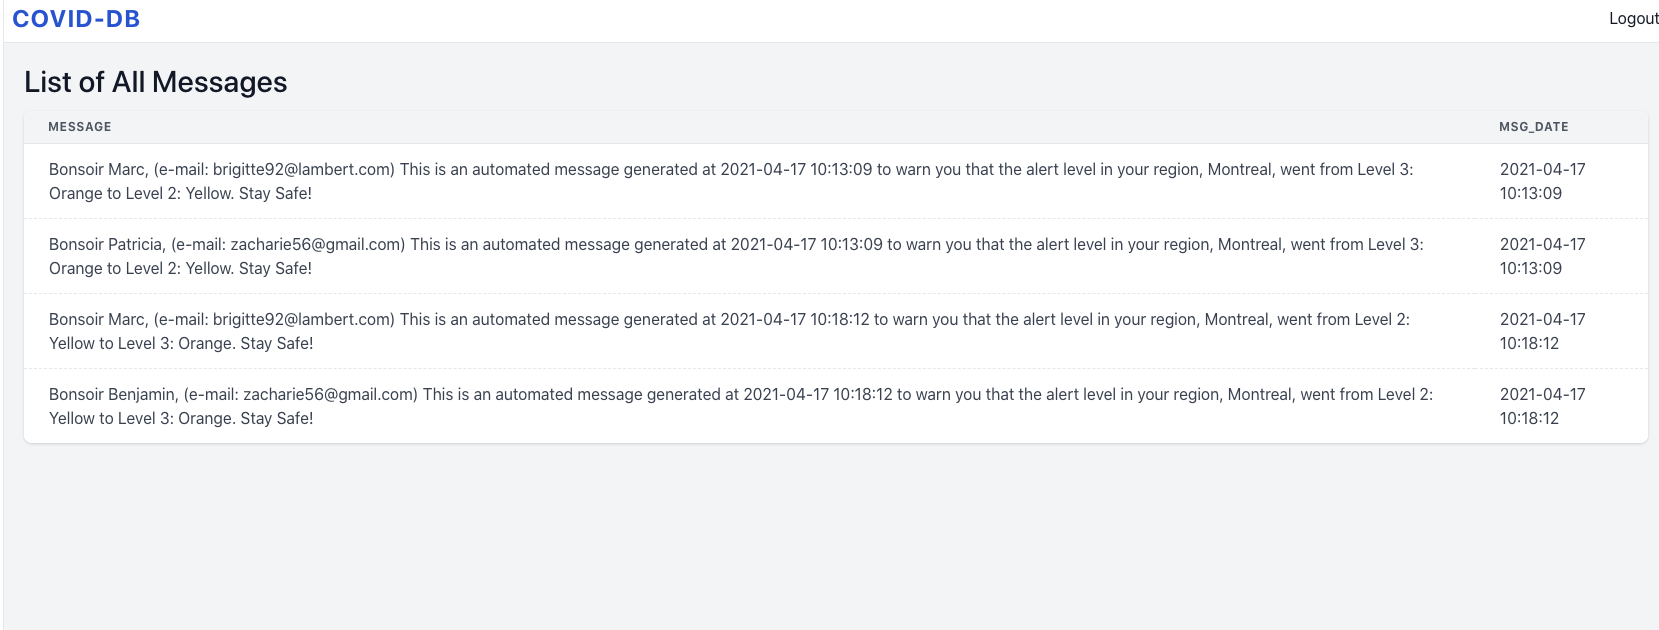
\includegraphics[scale=0.3]{imgs/allmsgs.png}
    \caption{Display all messages generate during in a given time}
\end{figure}

% Q11 %
\subsection{People in an address}
Give a list of all the People in a specific address. For every person, provide
the first name, last name, DOB, medicare card number, telephone number,
citizenship, email address, full mother’s name and full father’s name.
\subsubsection{MySQL}
\begin{minted}{MYSQL}
SELECT ps.first_name, ps.last_name, ps.dob, ps.medicare, ps.phone, ps.citizenship, ps.email,
group_concat(ps2.first_name , ' ', ps2.last_name) as parent_full_name FROM person ps
JOIN carer c ON c.child_id = ps.person_id
JOIN person ps2 ON c.parent_id = ps2.person_id
WHERE ps.address = '3239 Isaac Lake Apt. 198'
GROUP BY medicare;
\end{minted}

\subsubsection{PHP}
\begin{minted}{php}
<?php
public function readAll(Request $request)
{
    $criteria = collect();
    if ($request->filled('address')) {
        $criteria->put("address =  {$request->address}");
    }
    
    $stringQuery = $criteria->count() > 0 ? 'WHERE ' . $criteria->join(',');
    return response()->json(DB::select("SELECT p.patient_id, ps.*
        FROM Patient p
        JOIN Person ps ON p.person_id = ps.person_id $stringQuery"));
}
\end{minted}
\subsubsection{Representative tuples}
Which would return something like :
\begin{table}[ht]
\centering
    \begin{tabular}{|l|l|l|l|l|l|l|} 
        \hline
        first & last & dob & medicare & phone & citizenship & parent full \\
        \hline 
        Christine & Tessier & 1988-08-15 & YNPI68246266 & 18135950684 & US & Nathalie Roy, Jules Langlois\\
        Julie & Titty & 1969-04-20 & ADFY12346214 & 13953393929 & CA & Marcel Bo, Dom Nadeau \\
        Edith & Tardif & 1990-06-29 & GCPI16679278 & (730) 404-1566 & MX & Guillaume\\
        \hline
    \end{tabular}
    \caption{People living in the same address representative tuples.}
    \end{table}
\subsubsection{Screenshot in WebApp}   

\begin{figure}[H]
    \centering
    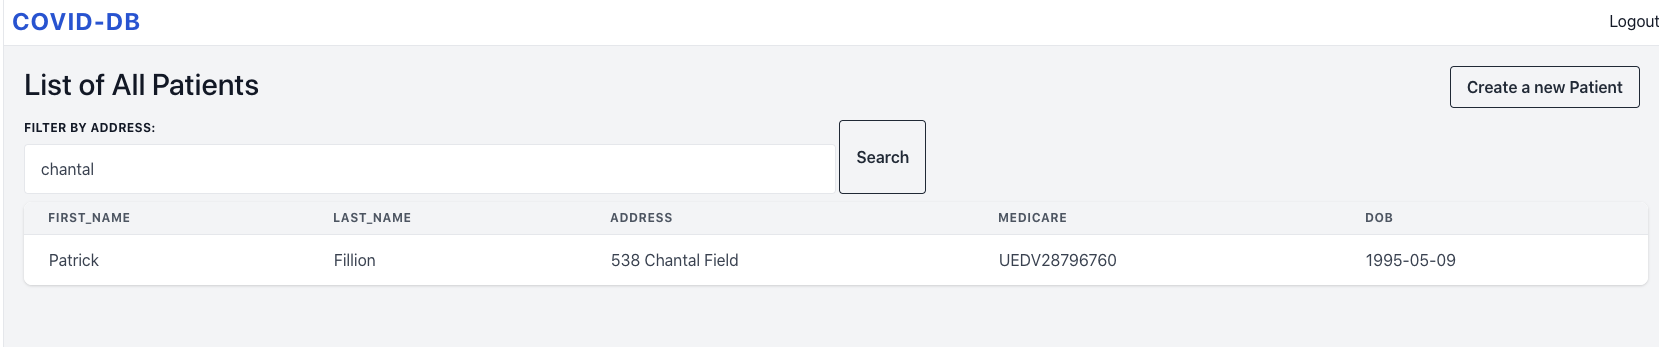
\includegraphics[scale=0.25]{imgs/patientsbyadr.png}
    \caption{Patients in an address}
\end{figure}



\subsection{Details of all facilities}
Give a detail list of all facilities (Address, Number of health workers, accept
walk-in clients or by appointment only, Drive thru capability, etc.).

\subsubsection{MySQL}
\begin{minted}{MYSQL}
SELECT
   phc.`health_center_id`,
   phc.`name`,
   phc.`phone`,
   phc.`address`,
   phc.`type`,
   phc.`method`,
   COUNT(w.health_worker_id) as 'worker_amount',
   if (phc.`drive_thru`, 'Yes','No')
FROM PublicHealthCenter phc
JOIN PublicHealthWorker w ON w.health_center_id = phc.health_center_id
GROUP BY phc.health_center_id

\end{minted}

\subsubsection{PHP}
\begin{minted}{php}
<?php
public function readAll(Request $request)
{
    return response()->json(DB::select("
        SELECT
               phc.`health_center_id`,
               phc.`name`,
               phc.`phone`,
               phc.`address`,
               phc.`type`,
               phc.`method`,
               COUNT(w.health_worker_id) as 'worker_amount',
               if (phc.`drive_thru`, 'Yes','No') as 'drive_thru'
        FROM PublicHealthCenter phc
        JOIN PublicHealthWorker w ON w.health_center_id = phc.health_center_id
        GROUP BY phc.health_center_id"));
}

\end{minted}

\subsubsection{Screenshot in webapp}

\begin{figure}[H]
    \centering
    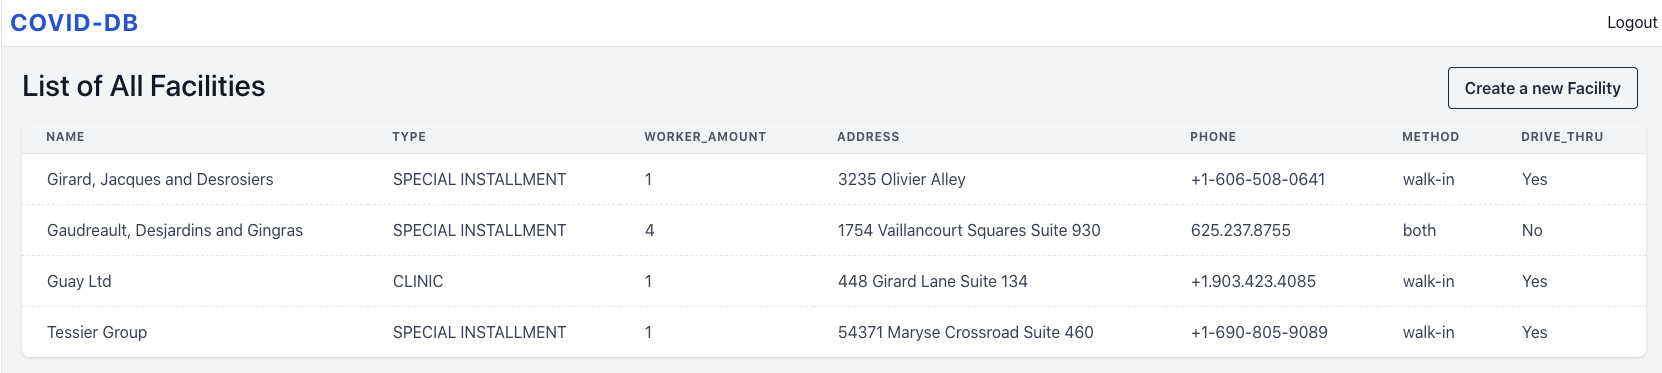
\includegraphics[scale=0.32]{imgs/allfacilities.png}
    \caption{Displaying details of all facilities}
\end{figure}

\subsection{Details of all Regions}
Give a detail list of all Regions (Name, list of all cities within the region,
and a list of all the postal codes within every city). 


\subsubsection{MySQL}
\begin{minted}{MYSQL}
SELECT
    r.region_id,
    r.region_name,
    a.alert_id,
    a.alert_info,
    count(p.person_id) as 'people_amount',
    GROUP_CONCAT(c.city) as 'cities',
    GROUP_CONCAT(pc.postal_code_id) as 'postal_codes'
FROM Region r
JOIN Alert a ON r.alert_id = a.alert_id
JOIN City c ON c.region_id = r.region_id
JOIN PostalCode pc ON pc.city_id = c.city_id
LEFT JOIN Person p ON p.postal_code_id = pc.postal_code_id
GROUP BY r.region_id ORDER BY count(p.person_id) DESC
\end{minted}

\subsubsection{PHP}
\begin{minted}{php}
<?php
public function readAll(Request $request)
{
    return response()->json(DB::select("
        SELECT
            r.region_id,
            r.region_name,
            a.alert_id,
            a.alert_info,
            count(p.person_id) as 'people_amount',
            GROUP_CONCAT(c.city) as 'cities',
            GROUP_CONCAT(pc.postal_code_id) as 'postal_codes'
        FROM Region r
        JOIN Alert a ON r.alert_id = a.alert_id
        JOIN City c ON c.region_id = r.region_id
        JOIN PostalCode pc ON pc.city_id = c.city_id
        LEFT JOIN Person p ON p.postal_code_id = pc.postal_code_id
        GROUP BY r.region_id ORDER BY count(p.person_id) DESC"));
}

\end{minted}

\subsubsection{Screenshot in Webapp}

\begin{figure}[H]
    \centering
    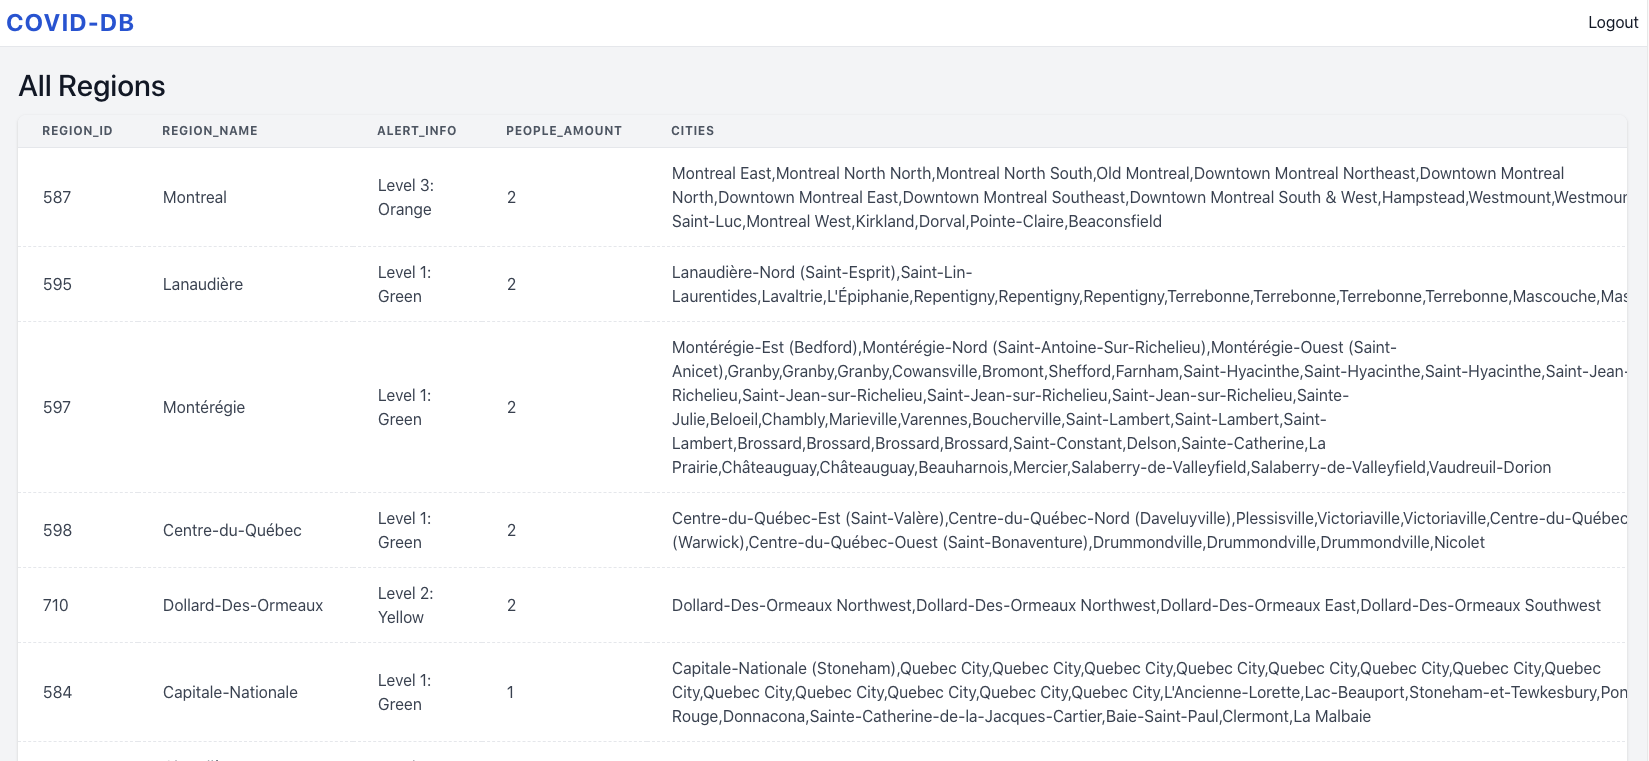
\includegraphics[scale=0.25]{imgs/allregions.png}
    \caption{Displaying details of all regions}
\end{figure}

\subsection{Details of people's test result in a date ordered by result}
Give a List of all people who got the result of the test on a specific date
(Date of the result of the test) grouped by the test result value (First who got
positive result, then who got negative result). The list must include First
Name, Last Name, DOB, Phone Number and email address of the diagnosed
person. 

\subsubsection{MySQL}
\begin{minted}{MYSQL}
SELECT ps.first_name, ps.last_name, ps.dob, ps.phone, ps.email, diagnostic_date, result
FROM diagnostic
NATURAL JOIN patient pt
NATURAL JOIN person ps
WHERE diagnostic_date > '2020-07-01 02:26:24'
ORDER BY result DESC;
\end{minted}

\subsection{List of all workers in a Facility}
Give a list of all workers in a specific facility. 

\subsubsection{MySQL}
\begin{minted}{MYSQL}
SELECT ps.first_name, ps.last_name, health_worker_id FROM publichealthworker
NATURAL JOIN Person ps
WHERE health_center_id = '3'
\end{minted}

\subsection{Workers with COVID at a facility on date and their reach}
Give a list of all public health workers who tested positive on a specific date
in a specific facility. In addition, provide a list of the employees who worked
with the infected health workers for the period of fourteen days prior to the
test. Use the date of the test taken by the infected health worker.

\subsubsection{MySQL}
\begin{minted}{MYSQL}
#6.9(1)
#ALL WORKERS WITH COVID ON THIS DATE AT THIS FACILITY
SELECT * FROM diagnostic
NATURAL JOIN patient pt
NATURAL JOIN person ps
JOIN publichealthworker pw ON pw.person_id = ps.person_id
WHERE result = '1' AND diagnostic_date > 0 AND pw.health_center_id = 2;

#6.9(2)
#RETURN WORKER THAT WORKS AT SAME FACILITY 
SELECT * FROM publichealthworker
WHERE health_center_id = 2
\end{minted}

\subsection{Report for every region}
For all regions, provide a report that include the region name, the number
of people who have positive results, the number of people who have
negative results and a history of alerts within a specific period-of- time. 

\subsubsection{MySQL}
\begin{minted}{MYSQL}
SELECT
    r.region_id,
    r.region_name,
    a.alert_id,
    a.alert_info,
    count(p.person_id) as 'people_amount',
    sum(if(aux.came_positive, 1, 0)) as amount_positive,
    sum(if(aux.came_positive, 0, 1)) as amount_negative,
    GROUP_CONCAT(c.city) as 'cities',
    GROUP_CONCAT(pc.postal_code_id) as 'postal_codes'
FROM Region r
JOIN Alert a ON r.alert_id = a.alert_id
JOIN City c ON c.region_id = r.region_id
JOIN PostalCode pc ON pc.city_id = c.city_id
LEFT JOIN Person p ON p.postal_code_id = pc.postal_code_id
LEFT JOIN (
    SELECT 
       pt.person_id as 'person_id',
       MAX(d.diagnostic_date) 'last_diagnostic_date',
       MAX(d.result) as 'came_positive'
    FROM Patient pt
      JOIN Diagnostic d ON pt.patient_id = d.patient_id
      GROUP BY pt.person_id
      ORDER BY MAX(d.diagnostic_date) 
) as aux ON aux.person_id = p.person_id
GROUP BY r.region_id ORDER BY count(p.person_id) DESC;
\end{minted}
